\section{Methodology}
\label{sec:method}

Figure~\ref{fig:framework_overview} presents an overview of our framework.
Our goal is not only to classify whether a meme is harmful, but also to produce a structured interpretation of the meme by identifying its target, intent, and tactic, together with the internal and external evidence that supports the prediction.
To this end, we decompose the problem into five stages:
(A) internal evidence extraction,
(B) external knowledge acquisition,
(C) knowledge relevance filtering and verification,
(D) evidence fusion and task-aware reasoning, and
(E) structured interpretation with evidence attribution.

\begin{figure*}[t]
    \centering
    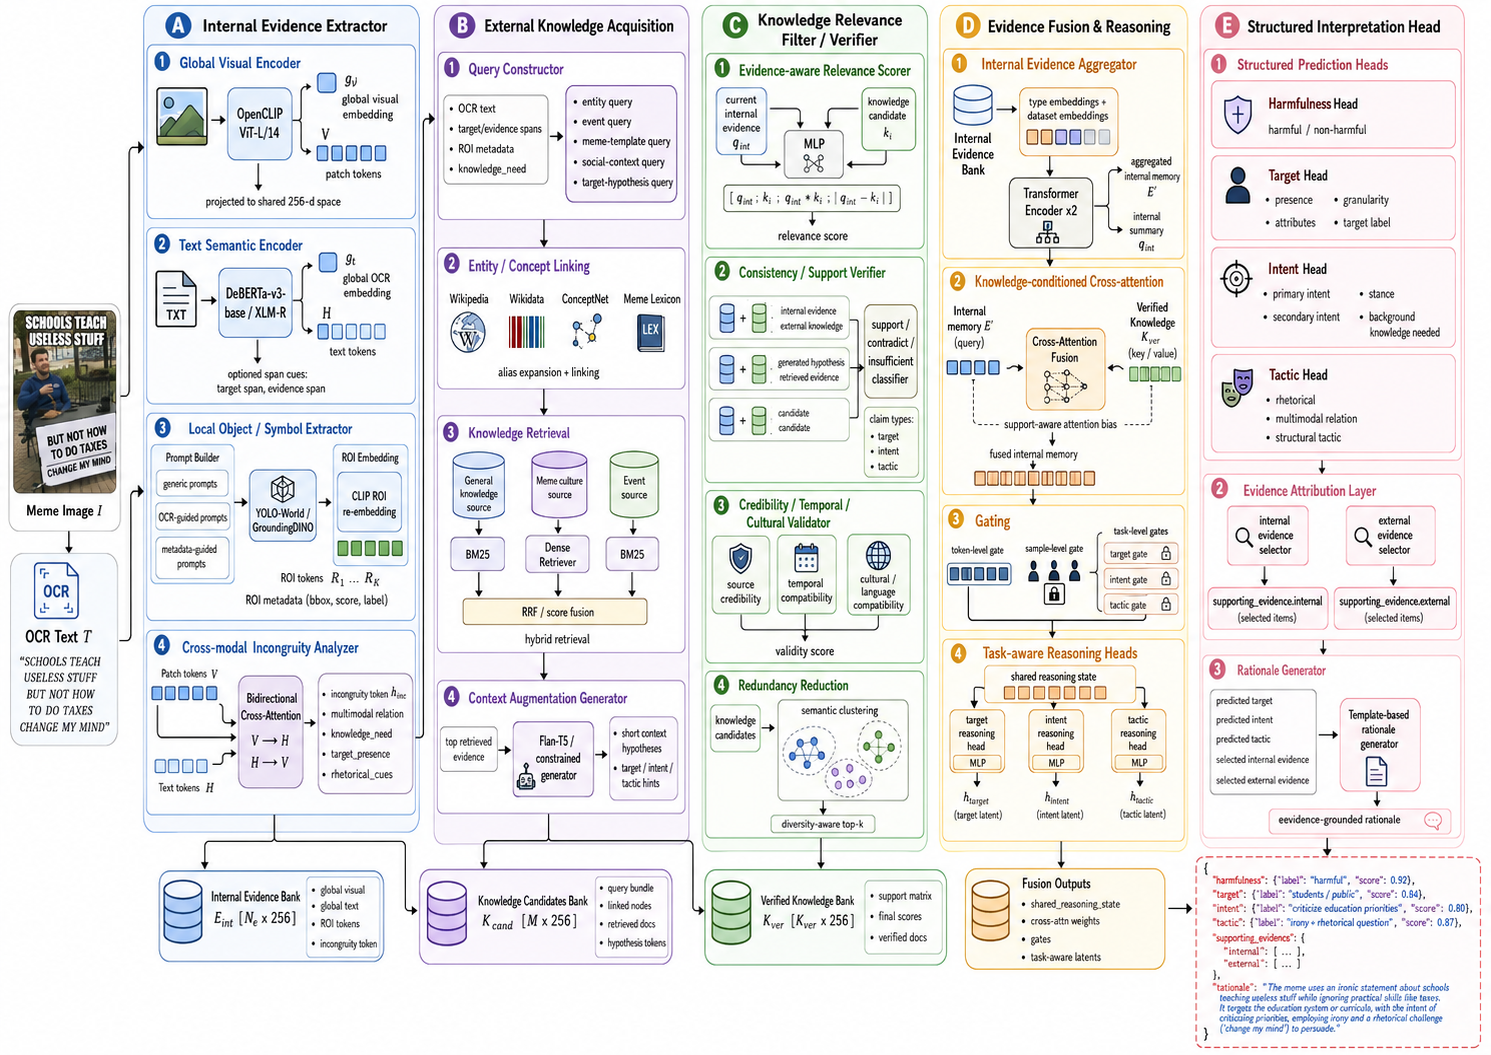
\includegraphics[width=\textwidth]{figures/manual/framework_architecture.png}
    \caption{
    Overview of our framework for evidence-grounded structured harmful meme interpretation.
    The framework consists of five stages:
    (A) internal evidence extraction,
    (B) external knowledge acquisition,
    (C) knowledge relevance filtering and verification,
    (D) evidence fusion and task-aware reasoning, and
    (E) structured interpretation with evidence attribution and rationale generation.
    This figure is a temporary project-stage visualization and will be replaced by the final camera-ready architecture figure.
    }
    \label{fig:framework_overview}
\end{figure*}

\subsection{Framework Overview}
\label{sec:method:overview}

Given a meme $\mathcal{M}=(I,T)$ consisting of an image $I$ and OCR text $T$, our framework first extracts internal evidence directly from the meme.
It then retrieves external contextual knowledge that may help interpret implicit targets, socio-cultural references, or event-dependent meanings.
Because retrieved knowledge is often noisy, outdated, or only weakly related to the meme, we explicitly filter and verify external candidates before using them.
The verified knowledge is fused with internal evidence through task-aware reasoning modules, and the final stage produces structured outputs for harmfulness, target, intent, and tactic, along with supporting evidence and an evidence-grounded rationale.

Formally, the overall pipeline can be written as

\begin{equation}
\mathcal{E}^{\mathrm{int}} = f_A(I,T),
\end{equation}

\begin{equation}
\mathcal{K}_{\mathrm{cand}} = f_B(I,T,\mathcal{E}^{\mathrm{int}}),
\end{equation}

\begin{equation}
\mathcal{K}_{\mathrm{ver}} = f_C(I,T,\mathcal{E}^{\mathrm{int}},\mathcal{K}_{\mathrm{cand}}),
\end{equation}

\begin{equation}
\mathbf{z} = f_D(\mathcal{E}^{\mathrm{int}},\mathcal{K}_{\mathrm{ver}}),
\end{equation}

\begin{equation}
\hat{\mathcal{Y}}, \hat{\mathcal{A}} = f_E(\mathbf{z}),
\end{equation}

where $\mathcal{E}^{\mathrm{int}}$ denotes internal evidence,
$\mathcal{K}_{\mathrm{cand}}$ denotes external knowledge candidates,
$\mathcal{K}_{\mathrm{ver}}$ denotes verified external knowledge,
$\mathbf{z}$ denotes fused task-aware latent representations,
$\hat{\mathcal{Y}}$ denotes structured predictions, and
$\hat{\mathcal{A}}$ denotes attribution outputs including selected evidence and rationale.

\subsection{Stage A: Internal Evidence Extractor}
\label{sec:method:stage_a}

The purpose of Stage A is to extract evidence directly observable from the meme itself.
This stage captures not only unimodal information from the image and text, but also localized symbolic cues and cross-modal incongruity patterns that are central to meme interpretation.

\paragraph{Global visual encoding.}
We first encode the meme image $I$ using a visual backbone to obtain a global visual representation and patch-level visual tokens:

\begin{equation}
\mathbf{g}_v, \mathbf{V} = \mathrm{VisualEncoder}(I),
\end{equation}

where $\mathbf{g}_v \in \mathbb{R}^{d}$ is the global image embedding and
$\mathbf{V} \in \mathbb{R}^{n_v \times d}$ is the set of patch tokens.

\paragraph{Text semantic encoding.}
The OCR text $T$ is encoded by a text encoder to produce a global text representation and token-level text embeddings:

\begin{equation}
\mathbf{g}_t, \mathbf{H} = \mathrm{TextEncoder}(T),
\end{equation}

where $\mathbf{g}_t \in \mathbb{R}^{d}$ is the global text embedding and
$\mathbf{H} \in \mathbb{R}^{n_t \times d}$ is the token sequence.

\paragraph{Local object and symbol extraction.}
Many harmful memes rely on localized visual cues such as logos, gestures, cultural symbols, or specific entities.
To capture such evidence, we apply region-level extraction and obtain a set of ROI tokens:

\begin{equation}
\mathbf{R} = \{ \mathbf{r}_1, \ldots, \mathbf{r}_K \}, \quad \mathbf{r}_k \in \mathbb{R}^{d}.
\end{equation}

Each ROI is associated with metadata such as bounding box, detector confidence, and tentative category label.

\paragraph{Cross-modal incongruity analysis.}
A key property of memes is that meaning often emerges from the tension between image and text rather than from either modality alone.
We therefore model cross-modal incongruity by allowing bidirectional interaction between visual and textual tokens:

\begin{equation}
\mathbf{C} = \mathrm{CrossModalAnalyzer}(\mathbf{V}, \mathbf{H}),
\end{equation}

where $\mathbf{C}$ denotes cross-modal evidence such as irony, contradiction, target cues, and rhetorical mismatch patterns.

Finally, Stage A outputs an internal evidence bank

\begin{equation}
\mathcal{E}^{\mathrm{int}} =
\left\{
\mathbf{g}_v, \mathbf{g}_t, \mathbf{V}, \mathbf{H}, \mathbf{R}, \mathbf{C}
\right\}.
\end{equation}

\subsection{Stage B: External Knowledge Acquisition}
\label{sec:method:stage_b}

Some memes cannot be interpreted reliably from internal content alone.
For example, the meme may reference a public event, a political actor, a culture-specific phrase, or a stereotype whose harmfulness depends on outside context.
Stage B therefore retrieves auxiliary contextual knowledge conditioned on the meme and the internal evidence extracted in Stage A.

\paragraph{Query construction.}
We build a query bundle from OCR text, detected entities, ROI metadata, target-related spans, and knowledge-need cues estimated from internal evidence.
This yields multiple query types, such as entity queries, event queries, social-context queries, and target-hypothesis queries.

\paragraph{Entity and concept linking.}
To improve retrieval specificity, extracted mentions are linked or expanded through entity and concept resources.
This step helps bridge lexical variation, aliases, and implicit references.

\paragraph{Knowledge retrieval.}
Given the query bundle, we retrieve candidate evidence from external sources.
The retriever may access general encyclopedic sources, meme-related culture resources, and event-oriented knowledge sources.
The retrieved results are aggregated into a candidate set

\begin{equation}
\mathcal{K}_{\mathrm{cand}} = \{ k_1, \ldots, k_M \}.
\end{equation}

\paragraph{Context augmentation generation.}
In addition to raw retrieved passages, we optionally generate short contextual hypotheses or compressed summaries that reformulate the retrieved evidence into meme-relevant interpretations.
These generated candidates are treated as knowledge candidates rather than trusted evidence.

\subsection{Stage C: Knowledge Relevance Filter / Verifier}
\label{sec:method:stage_c}

External retrieval is useful but noisy.
A candidate may be topically adjacent yet irrelevant to the meme, temporally outdated, culturally mismatched, or even contradictory to the meme’s actual implication.
Stage C explicitly verifies external knowledge before allowing it to influence downstream reasoning.

\paragraph{Evidence-aware relevance scoring.}
Each knowledge candidate $k_i$ is scored with respect to the current internal evidence:

\begin{equation}
s_i^{\mathrm{rel}} = \mathrm{RelScore}(\mathcal{E}^{\mathrm{int}}, k_i).
\end{equation}

This step estimates whether the candidate is genuinely relevant to the meme interpretation problem.

\paragraph{Consistency and support verification.}
Relevant candidates are then examined for whether they support, contradict, or insufficiently relate to the internal evidence and current task hypotheses.
This step is especially important because a retrieved passage may mention the same entity while still failing to support the intended target, intent, or tactic interpretation.

\paragraph{Credibility, temporal, and cultural validation.}
We further assess whether the source is credible and whether the information is temporally and culturally compatible with the meme context.
This is crucial for event-sensitive or community-specific memes.

\paragraph{Redundancy reduction.}
Finally, we cluster or rank candidates to reduce redundancy and retain a compact verified set:

\begin{equation}
\mathcal{K}_{\mathrm{ver}} \subseteq \mathcal{K}_{\mathrm{cand}}.
\end{equation}

The verified knowledge bank preserves provenance metadata such as origin, score, and support type, enabling later attribution.

\subsection{Stage D: Evidence Fusion and Task-Aware Reasoning}
\label{sec:method:stage_d}

Stage D combines internal evidence and verified external knowledge into task-sensitive latent representations.
Rather than fusing all information uniformly, we adopt a task-aware reasoning design because harmfulness, target identification, intent inference, and tactic recognition often depend on different subsets of evidence.

\paragraph{Internal evidence aggregation.}
Internal evidence is first aggregated into a contextual memory representation:

\begin{equation}
\mathbf{E}^{\mathrm{int}} = \mathrm{AggInt}(\mathcal{E}^{\mathrm{int}}).
\end{equation}

\paragraph{Knowledge-conditioned cross-attention.}
We then fuse internal memory with verified knowledge through cross-attention:

\begin{equation}
\mathbf{E}^{\mathrm{fused}} =
\mathrm{CrossAttn}(\mathbf{E}^{\mathrm{int}}, \mathcal{K}_{\mathrm{ver}}).
\end{equation}

This allows the model to selectively integrate contextual knowledge where it improves interpretation.

\paragraph{Task-aware gating.}
Not all tasks require the same amount or type of evidence.
For example, harmfulness may often rely on broad multimodal signals, whereas target interpretation may depend more strongly on entity-level or background cues.
We therefore use gating functions that modulate evidence flow at token, sample, and task levels:

\begin{equation}
\mathbf{z}^{(q)} = \mathrm{Gate}_q(\mathbf{E}^{\mathrm{fused}}), \quad q \in \mathcal{Q},
\end{equation}

where $\mathcal{Q}$ denotes the task set.

\paragraph{Task-aware reasoning heads.}
From the gated shared memory, we derive task-specific latent states for target-, intent-, and tactic-oriented reasoning.
These latent states are not yet final predictions; rather, they provide specialized representations used by the structured interpretation head.

\subsection{Stage E: Structured Interpretation Head}
\label{sec:method:stage_e}

Stage E converts the fused task-aware representations into structured predictions, evidence attribution outputs, and a concise rationale.

\paragraph{Structured prediction heads.}
We use dedicated output heads for harmfulness, target, intent, and tactic.
These heads jointly produce the structured output defined in Section~\ref{sec:problem}.
Concretely, the framework predicts:
(i) harmfulness,
(ii) target presence and target granularity,
(iii) primary intent, and
(iv) rhetorical tactic and multimodal relation.

\paragraph{Evidence attribution layer.}
To improve interpretability, we separately select supporting internal and external evidence for each prediction.
This yields attribution sets such as

\begin{equation}
\hat{\mathcal{A}}^{\mathrm{int}} \subseteq \mathcal{E}^{\mathrm{int}},
\qquad
\hat{\mathcal{A}}^{\mathrm{ext}} \subseteq \mathcal{K}_{\mathrm{ver}}.
\end{equation}

These selected items are serialized as supporting evidence rather than only being used implicitly inside the model.

\paragraph{Rationale generation.}
Finally, we generate a concise rationale conditioned on the predicted labels and selected evidence.
The rationale is designed to summarize why the meme was interpreted in a particular way, while remaining grounded in the extracted evidence and verified knowledge.

\subsection{Training Objective}
\label{sec:method:training}

The framework is trained in a multi-task manner.
Let $\mathcal{Q}$ denote the set of supervised tasks and let $m_n^q$ be a binary supervision mask indicating whether task $q$ is valid for sample $n$.
The overall objective is

\begin{equation}
\mathcal{L}
=
\sum_{q \in \mathcal{Q}}
\lambda_q \mathcal{L}_q,
\end{equation}

where $\lambda_q$ is the task weight and $\mathcal{L}_q$ is the loss for task $q$.
We use cross-entropy losses for single-label tasks and binary cross-entropy for multi-label rhetorical tactic prediction.
Masked supervision is applied so that ignored or unavailable labels do not contribute to the loss.

In addition to prediction outputs, the framework preserves structured metadata about evidence provenance, gating behavior, and attribution sources.
These records are not treated as primary prediction targets, but they are essential for later auditing, error analysis, and evidence-grounded evaluation.